\chapter{من تكاملات المسار إلى المروِّجات والرؤوس}

قبل الانتقال إلى استعراض الجسيمات وتآثراتها، يجدر توضيح البناء المركزي. فاللاجرانجي يفعل أكثر من مجرد ترميز معادلات الحقل الكلاسيكية. فمن خلال تكامل المسار يوفّر أيضًا سعاتٍ لانتشار الجسيمات وانشطارها والتحامها وتشتتها. وهذا هو الطريق الأكثر مباشرة من نظرية الحقل الكمومي إلى مخططات فينمان.

\section{مبدأ الفعل الأصغر للجسيمات والحقول}

تكامل المسار لدى فينمان هو النظير الكمومي لمبدأ الفعل الأصغر. ابدأ بجسيم نيوتني عادي، يعتمد لاجرانجيه على إحداثياته وسرعاته،
\begin{equation}
\mathcal{L}=\mathcal{L}(x,\dot{x}),
\end{equation}
والفعل المسند إلى مسار هو
\begin{equation}
S[x]=\int \mathcal{L}(x,\dot{x})\,dt.
\end{equation}
لكل مسار مرشَّح من نقطة في الزمكان إلى أخرى فعلٌ، سواء استوفى معادلات نيوتن أم لا. ويتميّز المسار الكلاسيكي بأن الفعل ساكن عنده. وفي اللغة التقليدية ``للفعل الأصغر'' يُقال إنه يصغِّر الفعل، مع أن السكونية هي العبارة الأعم. ويعطي شرط السكونية المعادلات التفاضلية الكلاسيكية للحركة.

\begin{figure}[htbp]
\centering
\includegraphics[width=0.72\textwidth]{lecture_10_figure_02.png}
\caption{تكامل الفعل لمسار جسيم.}
\lectureframe{00:02:14}
\end{figure}

تنطبق البنية نفسها على حقل كلاسيكي. ومثّل جميع الحقول على نحو عام بالرمز \(\phi\). وقد تعتمد كثافة لاجرانجي محلية للحقل على الحقول وعلى مشتقاتها المكانية والزمانية معًا:
\begin{equation}
\mathcal{L}
=\mathcal{L}\!\left(\phi,\frac{\partial\phi}{\partial x^\mu}\right)
=\mathcal{L}(\phi,\partial_\mu\phi).
\end{equation}
وتقتضي النسبية أن يتحول \(\mathcal{L}\) على أنه مقدار قياسي لورنتزي. ومع مراعاة هذا الشرط، فإن التراكيب القياسية المبنية من الحقول ومشتقاتها تعطي الحدود الممكنة في اللاجرانجي.

\begin{figure}[htbp]
\centering
\includegraphics[width=0.62\textwidth]{lecture_10_figure_03.png}
\caption{اعتماد لاجرانجي الحقل على الحقل وعلى مشتقاته الزمكانية.}
\lectureframe{00:04:09}
\end{figure}

بالنسبة إلى الحقل، يُكامل الفعل على منطقة من الزمكان:
\begin{equation}
S[\phi]=\int_{\Omega} d^4x\,\mathcal{L}(\phi,\partial_\mu\phi),
\qquad
d^4x=dt\,dx\,dy\,dz.
\end{equation}
فعل الجسيم تكامل على الزمن على طول مسار. أما فعل الحقل فهو كثافة لاجرانجي مكاملة في أرجاء منطقة زمكانية بأكملها.

ونظير تثبيت نقطتي نهاية مسار جسيم هو تعيين تهيئة الحقل الكاملة على شريحة زمنية ابتدائية وعلى شريحة زمنية نهائية. فإذا كان الحقل الابتدائي هو \(\phi_{\mathrm{i}}(\mathbf{x})\) وكان الحقل النهائي هو \(\phi_{\mathrm{f}}(\mathbf{x})\)، فإن حقلًا وسيطًا يملأ الحيّز كله بينهما. وعندما تسمح معطيات الحد بوجود حل كلاسيكي وسيط، يكون ذلك الحل نقطة سكون للفعل مع تثبيت التهيئتين الحدّيتين.
\editorialnote{قد لا تسمح تهيئات حقل كاملة اعتباطية على شريحتين زمنيتين بوجود حل كلاسيكي. ولذلك فإن عبارة الفعل الساكن مقصورة على معطيات حدية يوجد لها حل وسيط.}

هذا الشكل الهندسي هو النظير في نظرية الحقل لمسار الجسيم.\footnote{أُعيد بناء اللوح الزمكاني من الرسم عند نحو 00:04:29.}
\begin{figure}[htbp]
\centering
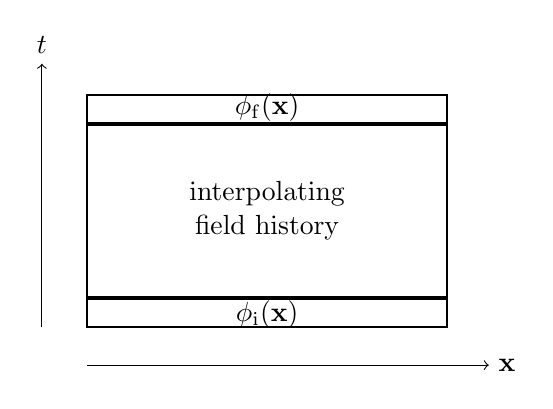
\begin{tikzpicture}[scale=0.88]
\draw[->] (-0.65,0) -- (-0.65,3.8) node[above] {$t$};
\draw[->] (0,-0.55) -- (5.8,-0.55) node[right] {$\mathbf{x}$};
\draw[thick] (0,0) rectangle (5.2,3.35);
\draw[very thick] (0,0.42) -- (5.2,0.42);
\draw[very thick] (0,2.93) -- (5.2,2.93);
\node at (2.6,0.18) {$\phi_{\mathrm{i}}(\mathbf{x})$};
\node at (2.6,3.17) {$\phi_{\mathrm{f}}(\mathbf{x})$};
\node[align=center] at (2.6,1.68) {interpolating\\field history};
\end{tikzpicture}
\caption{تهيئتا الحقل الابتدائية والنهائية اللتان تحدّان منطقة زمكانية.}
\end{figure}

\begin{classroomqa}
\lecturetimestamp{00:07:34}
\audiencequestion{هل يمكن لحقل أن يعود إلى القيمة نفسها؟}
\lecturerresponse{نعم. لا يوجد ما يمنع حقلًا من العودة إلى قيمة سابقة، كما لا يوجد ما يمنع إحداثي جسيم من العودة إلى موضع سابق.}
\end{classroomqa}

\begin{classroomqa}
\lecturetimestamp{00:07:46}
\audiencequestion{لماذا نتحدث عن أحداث زمكانية أو عن مسار بينما معطيات الحد هي قيم الحقل؟}
\lecturerresponse{يُستبدل بمسار الجسيم تاريخ حقلي. فكل نقطة نهاية في فضاء الحقول هي الحقل بأكمله على شريحة زمنية مختارة، ويحدِّد تاريخ واحد الحقل عند كل نقطة في المنطقة الزمكانية بين الشريحتين.}
\end{classroomqa}

إن اشتراط سكونية الفعل للحقل الوسيط ينتج معادلات تفاضلية جزئية. واعتمادًا على الحقول واللاجرانجي، تشمل هذه المعادلات معادلاتٍ مثل معادلات ماكسويل، ولفعلٍ ثقالي، معادلات أينشتاين. ولا نحتاج هنا إلى الاشتقاق التغايري التفصيلي؛ فالتسلسل المهم هو
\begin{equation}
\mathcal{L}
\longrightarrow
S[\phi]
\longrightarrow
\text{classical field equations}.
\end{equation}

\section{مجموع فينمان على مسارات الجسيمات}

تستبدل ميكانيكا الكم السؤال عن أيِّ مسار يحدث بسؤال عن السعات. تخيّل إدخال جسيم عند \((x,t)\)، ثم إغماض العينين برهة، ثم تشغيل كاشف عند \((x',t')\). والسعة
\begin{equation}
\mathcal{A}(x,t;x',t')
\end{equation}
عدد مركب. ومربع مقدارها هو الاحتمال:
\begin{equation}
\begin{aligned}
P(x,t;x',t')
&=\left|\mathcal{A}(x,t;x',t')\right|^2\\
&=\mathcal{A}(x,t;x',t')
\mathcal{A}(x,t;x',t')^*.
\end{aligned}
\end{equation}

تنسب قاعدة فينمان فعلًا إلى كل مسار مرشَّح، وتربط به الطور
\begin{equation}
\exp\!\left(-\frac{i}{\hbar}S[x]\right)
=
\exp\!\left[-\frac{i}{\hbar}\int \mathcal{L}(x,\dot{x})\,dt\right].
\end{equation}

\begin{figure}[htbp]
\centering
\includegraphics[width=0.70\textwidth]{lecture_10_figure_04.png}
\caption{الطور المركب المقترن بمسار جسيم.}
\lectureframe{00:11:52}
\end{figure}

يلزم العامل \(\hbar\) لكي يكون الأس بلا أبعاد.\footnote{عند 00:11:52 تُقرأ الصيغة على السبورة طبيعيًا على أنها \(e^{-i\int\mathcal{L}\,dt}\)؛ ويُذكر عامل \(\hbar\) شفهيًا عند 00:12:02.} وسعة الانتقال هي مجموع هذه الأطوار على كل مسار ممكن يصل بين النهايتين:
\begin{equation}
\mathcal{A}(x,t;x',t')
=
\sum_{\substack{\text{paths }x(\tau)\\(x,t)\rightarrow(x',t')}}
\exp\!\left(-\frac{i}{\hbar}S[x]\right).
\end{equation}
وهنا لا تعني عبارة ``مسار ممكن'' حلًا لمعادلات نيوتن، بل تعني أي مسار داخل في المجموع. وفي ميكانيكا الكم غير النسبية تتقدم المسارات إلى الأمام في الزمن بدلًا من الالتفاف إلى الخلف. ولثابت بلانك أبعاد الفعل، لذا فإن \(S/\hbar\) بلا أبعاد.

والدالة الأسية هنا طبيعية لأن سعات الخطوات الصغيرة المتعاقبة تتكاثر ضربًا. فإذا قُسِّم مسار إلى أجزاء متتالية، فإن الفعل يتجمع جمعًا،
\begin{equation}
S=S_1+S_2+\cdots,
\end{equation}
بينما تتكاثر الأطوار ضربًا:
\begin{equation}
e^{-iS/\hbar}
=e^{-iS_1/\hbar}e^{-iS_2/\hbar}\cdots.
\end{equation}
وليس العامل \(i\) مجرد أداة تدوين حسابي؛ بل هو جزء من القاعدة الكمومية.

\begin{classroomqa}
\lecturetimestamp{00:13:27}
\audiencequestion{هل ترتبط الدالة الأسية بضرب سعات الخطوات الصغيرة المتعاقبة؟}
\lecturerresponse{نعم. سعات الخطوات المتعاقبة تتكاثر ضربًا، في حين أن الأجزاء المناظرة من الفعل تتجمع جمعًا.}
\end{classroomqa}

\begin{classroomqa}
\lecturetimestamp{00:13:49}
\audiencequestion{هل المجموع على المسارات هو نفسه الاحتمال؟}
\lecturerresponse{لا. مجموع المسارات هو سعة احتمال تكون عمومًا مركبة. ويعطي ضربها في مرافقها المركب الاحتمال.}
\end{classroomqa}

\section{المجموع على تواريخ الحقول}

ويمتد هذا الصوغ نفسه إلى نظرية الحقل الكمومي، وإن كان البناء هنا سيبقى عن قصد غير صارم. ابدأ بتهيئة حقل ابتدائية \(\phi(\mathbf{x})\) وبتهيئة نهائية محددة على نحو مستقل \(\phi'(\mathbf{x})\). وهاتان دالتان كاملتان في المكان، لا قيمتان عند نقطتين معزولتين.

يمكن تخيّل جهاز مثالي يهيِّئ الحقل عند كل نقطة مكانية، ثم يترك النظام يتطور، ثم يقيس الحقل لاحقًا عند كل نقطة. ومثل هذا الجهاز غير واقعي، لكنه يحدِّد السؤال المفهومي بوضوح: ما السعة للانتقال من تهيئة الحقل الكاملة الابتدائية إلى النهائية؟

يسهم كل تاريخ حقلي وسيط يمكن تخيّله. ولكل تاريخ، احسب
\begin{equation}
S[\phi]=\int d^4x\,\mathcal{L}(\phi,\partial_\mu\phi)
\end{equation}
وألحق به الطور الموافق. وعلى نحو تخطيطي،
\begin{equation}
\mathcal{A}\!\left[\phi(\mathbf{x})\rightarrow\phi'(\mathbf{x})\right]
=
\sum_{\substack{\text{field histories}\\
\phi_{\mathrm{i}}=\phi,\;\phi_{\mathrm{f}}=\phi'}}
\exp\!\left(-\frac{i}{\hbar}S[\phi]\right).
\end{equation}
ولا يلزم أن يحلَّ أي تاريخ معادلات الحقل الكلاسيكية. إنه ببساطة تعيين كامل واحد لقيم الحقل في جميع أنحاء المنطقة الزمكانية الفاصلة.

\begin{classroomqa}
\lecturetimestamp{00:17:39}
\audiencequestion{هناك عدد لا نهائي من التواريخ، ولكل طور مقدار يساوي الواحد. فكيف يمكن أن يتقارب مجموعها؟ وهل يجري تصغير هذه التواريخ؟}
\lecturerresponse{التواريخ تُجمع، لا تُصغَّر. فالحدود أطوار موزعة حول دائرة الوحدة، ولذا يمكن أن يُلغي بعضها بعضًا. وهذا يختلف عن جمع عدد لا نهائي من الحدود الموجبة التي تبقى بعيدة عن الصفر. ويمكن للتكاملات التذبذبية أن تتقارب؛ والتمثيل الفورييري لدالة دلتا مثال مألوف. ولو توزعت الأطوار بانتظام حول الدائرة، لانعدم مجموعها المتجهي. ومعظم التواريخ يُلغي بعضها بعضًا بقوة. أما التواريخ القريبة من تاريخ ذي فعل ساكن فيكون الإلغاء بينها أضعف، لأن الطور يتغير هناك بأبطأ معدل، وهكذا يظهر الحد الكلاسيكي.}
\end{classroomqa}

\editorialnote{يتطلب تكامل المسار في الزمن الحقيقي عادةً وصفةً للتقارب. ويقدِّم نقاش دائرة الوحدة هنا حجة الإلغاء التذبذبي المستخدمة في هذا الموضع، لا برهانًا عامًا على التقارب.}

يمكن تصوير هذا الإلغاء على أنه مجموع متجهات في المستوى المركب.\footnote{أُعيد بناء إنشاء دائرة الوحدة من مناقشة السبورة عند 00:18:32--00:20:21.}
\begin{figure}[htbp]
\centering
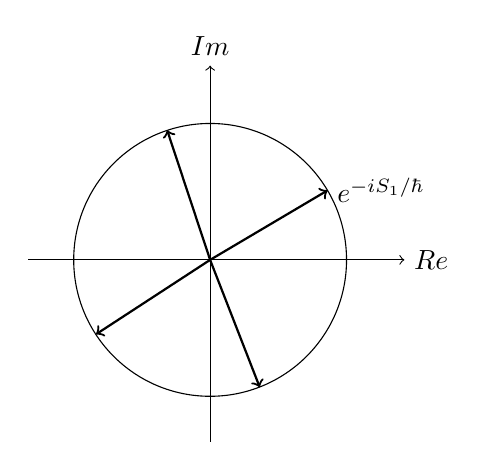
\begin{tikzpicture}[scale=1.05]
\draw[->] (-2.2,0) -- (2.35,0) node[right] {$\operatorname{Re}$};
\draw[->] (0,-2.2) -- (0,2.35) node[above] {$\operatorname{Im}$};
\draw (0,0) circle (1.65);
\draw[thick,->] (0,0) -- (1.42,0.84);
\draw[thick,->] (0,0) -- (-1.38,-0.90);
\draw[thick,->] (0,0) -- (-0.52,1.57);
\draw[thick,->] (0,0) -- (0.60,-1.54);
\node[right] at (1.42,0.84) {$e^{-iS_1/\hbar}$};
\end{tikzpicture}
\caption{يمكن للأطوار ذات المقدار الواحد أن يُلغي بعضها بعضًا عندما تختلف اتجاهاتها.}
\end{figure}

بل إن،
\begin{equation}
e^{-iS/\hbar}
=
\cos\!\left(\frac{S}{\hbar}\right)
-i\sin\!\left(\frac{S}{\hbar}\right).
\end{equation}
كل إسهام متجه وحدة. والإسهامات التي تتجه في اتجاهات مختلفة يطرح بعضها بعضًا كما يجمع بعضها بعضًا. وقرب نقطة سكون لـ \(S\)، يكون للتواريخ القريبة الطور نفسه تقريبًا، ولذلك تعزّز إسهاماتها بعضها بعضًا على نحو أكثر فاعلية. وبعيدًا عن الفعل الساكن، يتغير الطور بسرعة ويهيمن التداخل الهدام.

تقع بنية تكامل المسار هذه في أساس نظرية الحقل الكمومي الحديثة كلها تقريبًا. وستُذكر الخطوة العملية التالية بدلًا من اشتقاقها. وهذا مسلك مفرط في التبسيط إلى الحساب، لكنه يُظهر كيف يمكن استعمال الشيء نفسه بلغتين.

إن حساب عملية ما هو حساب احتمال انتقال من حالة ابتدائية إلى حالة نهائية. أحد الوصفين يحدد تهيئة حقلية ابتدائية وتهيئة حقلية نهائية. والوصف الآخر يحدد جسيمات داخلة وجسيمات خارجة، أي كوانتا حقل واحد أو عدة حقول. تبدو هاتان المسألتان مختلفتين، لكن كلتيهما تُحسب من تكامل المسار نفسه في نظرية الحقل.

\section{صيغة متقطعة للزمكان}

ولإعطاء المجموع على تواريخ الحقل معنىً ملموسًا، قسّم الزمكان إلى خلايا صغيرة وأسند قيمة حقلية إلى كل خلية. ويُقترب من حد الاستمرار بتصغير حجم الخلية، لكن الخلايا تبقى في الوقت الحاضر منتهية الحجم. وهذا يحوّل المجموع الصوري على الدوال إلى مجموع على إسناد أعداد إلى خلايا الشبكة.

يستعمل تقريب حدسي سابق حاصلَ ضرب لعوامل تشبه \(1+\mathcal{L}_i\)، عاملًا واحدًا لكل خلية، ثم يميّز الحدود التي تصف انتشار الجسيمات وتصادمها. وهذا البناء من الأهمية بحيث يستحق التكرار، لكن يجب تصحيح العامل. فالكمية الصغيرة ليست اللاغرانجيان نفسه، بل الفعل المحتوى في خلية.

إذا كان للخلية حجم زمكاني
\begin{equation}
a^4=\Delta t\,\Delta x\,\Delta y\,\Delta z,
\end{equation}
فإن فعلها هو
\begin{equation}
A_i=\mathcal{L}_i a^4.
\end{equation}
وبما أن الخلية صغيرة، فإن \(A_i\) صغير. ومع إهمال \(\hbar\) مؤقتًا، يكون العامل الأولي المصحح
\begin{equation}
1-iA_i,
\end{equation}
بدلًا من \(1+\mathcal{L}_i\).

لأي \(\epsilon\) صغير،
\begin{equation}
1+\epsilon\simeq e^\epsilon,
\end{equation}
وذلك لأن
\begin{equation}
e^\epsilon
=1+\epsilon+\frac{\epsilon^2}{2!}
+\frac{\epsilon^3}{3!}+\cdots.
\end{equation}
ومن ثم، في هذه الوحدات المؤقتة، يقارب \(1-iA_i\) المقدار \(e^{-iA_i}\) إذا كانت الخلية صغيرة بما يكفي. ومن الأنظف استعمال العامل الأسي الدقيق منذ البداية.

\begin{classroomqa}
\lecturetimestamp{00:27:57}
\audiencequestion{هل يتطلب العامل الأسي عاملًا من \(\hbar\)؟}
\lecturerresponse{نعم. عامل الخلية اللابعدي هو \(1-iA_i/\hbar\) في الرتبة الأولى، والعامل الأسي الدقيق هو \(\exp(-iA_i/\hbar)\). ويمكن لاحقًا اعتماد وحدات يكون فيها \(\hbar=1\).}
\end{classroomqa}

وبإرجاع \(\hbar\)، يكون العامل الوسيط المصحح وصيغته الأسية هما
\begin{equation}
1-\frac{i}{\hbar}A_i
\simeq
\exp\!\left(-\frac{i}{\hbar}A_i\right).
\end{equation}

من أجل تاريخ ثابت، استبدل تكامل الزمكان بمجموع أفعال الخلايا:
\begin{equation}
S[\phi]
=\int d^4x\,\mathcal{L}
\;\longrightarrow\;
\sum_i A_i.
\end{equation}
وعندئذٍ يصبح عامل الطور لذلك التاريخ
\begin{equation}
\exp\!\left(-\frac{i}{\hbar}\sum_i A_i\right).
\end{equation}
والعامل الأسي لمجموع يساوي حاصل ضرب العوامل الأسية:
\begin{equation}
\exp\!\left(-\frac{i}{\hbar}\sum_i A_i\right)
=
\prod_i\exp\!\left(-\frac{i}{\hbar}A_i\right).
\end{equation}
وترتيب العمليات مهم. اختر أولًا تاريخًا كاملًا واحدًا واضرب أوزان خلاياه. وعندئذ فقط اجمع على التواريخ المختلفة.

كما تجعل الشبكة معطيات الحدود صريحة.\footnote{أُعيد بناء رقعة الشطرنج وصفّيها الأول والأخير المثبَّتين من الرسوم عند نحو 00:23:54 و00:30:49.}
\begin{figure}[htbp]
\centering
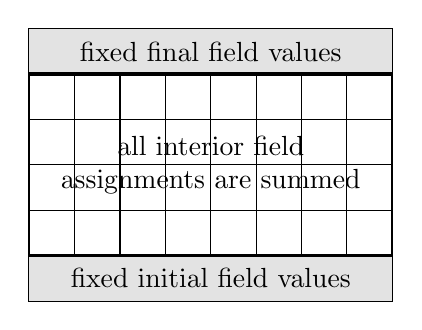
\begin{tikzpicture}[scale=0.72]
\draw[step=0.8,thin] (0,0) grid (6.4,4.8);
\draw[thick] (0,0) rectangle (6.4,4.8);
\fill[gray!22] (0,0) rectangle (6.4,0.8);
\fill[gray!22] (0,4.0) rectangle (6.4,4.8);
\draw[very thick] (0,0.8) -- (6.4,0.8);
\draw[very thick] (0,4.0) -- (6.4,4.0);
\node at (3.2,0.4) {fixed initial field values};
\node at (3.2,4.4) {fixed final field values};
\node[align=center] at (3.2,2.4) {all interior field\\assignments are summed};
\end{tikzpicture}
\caption{تواريخ حقلية متقطعة ذات صفين شبكيين ابتدائي ونهائي مثبتين.}
\end{figure}

يحدد الصف الأول تهيئة الحقل الابتدائية، ويحدد الصف الأخير التهيئة النهائية. ويُسمح لكل خلية داخلية بكل قيمة حقلية تدخل في التقطيع. وهكذا تأخذ سعة الانتقال الصيغة التخطيطية
\begin{equation}
\mathcal{A}\!\left[\phi_{\mathrm{i}}\rightarrow\phi_{\mathrm{f}}\right]
=
\sum_{\{\phi\}_{\mathrm{interior}}}
\prod_i\exp\!\left(-\frac{i}{\hbar}A_i[\phi]\right),
\end{equation}
مع إبقاء الصفين الأول والأخير ثابتين. وبصورة مكافئة، يُحسب لكل إسناد داخلي العامل الأسي للفعل الكلي، ثم تُضاف تلك المساهمة إلى مساهمات جميع الإسنادات الأخرى.

\section{من تهيئات الحقول إلى تهيئات الجسيمات}

يمكن وصف سعة الانتقال نفسها بدلالة الحقول أو بدلالة الجسيمات. فبدلًا من تثبيت الحقل على الشريحتين الزمنيتين الأولى والأخيرة، يمكن تحديد مجموعة داخلة من كوانتا الحقل ومجموعة خارجة من كوانتا الحقل، ثم السؤال عن السعة التي تصل بينهما. والشيء الجاري تقييمه هو نفسه. إنما الذي تغيّر هو وصف الحدود.

تحتوي الحقول الكمومية على مؤثرات إنشاء وإفناء. ولذلك تؤثر جداءات الحقول في حالات الجسيمات بإنشاء الكوانتا أو إفنائها أو نقلها. وهذه القراءة من حيث المؤثرات هي التي تحوّل تكامل المسار الشبكي إلى مجموعة من قواعد الجسيمات.

\begin{classroomqa}
\lecturetimestamp{00:34:11}
\audiencequestion{هل يمكن بالضرورة التعرف على كوانتا الحقل بوصفها جسيمات؟}
\lecturerresponse{ليس دائمًا بالمعنى التقليدي لجسيمات يمكن رصد كل منها على حدة. فالكواركات، مثلًا، هي كوانتا حقول الكوارك، لكن الحبس يمنع الكوارك المنعزل من الإفلات ومن أن يُكتشف وحده. وعلى نحو أعم، لا يلزم أن يوجد تقابل واحد لواحد بين الحقول المسمّاة في نظرية ما وأنواع الجسيمات التي تظهر بوصفها حالات قابلة للرصد بالمعنى التقليدي. وبعض نظريات الحقول لا تسمح بهذا التقابل البسيط. وإذا استُعمل ``جسيم'' بمعنى واسع يدل على كمّ غير قابل للانقسام يحمل طاقة وأعدادًا كمومية أخرى، فقد يصبح التمييز عندئذٍ جزئيًا مسألة اصطلاح.}
\end{classroomqa}

\editorialnote{العبارة المتعلقة بالاقتران الضعيف في المصدر عند 00:35:45--00:36:08 ملتبسة نحويًا، وتُترك هنا من دون حسم. أما الدعوى الموثوقة فهي أن تسميات الحقول وأنواع الجسيمات القابلة للرصد على نحو تقليدي لا يلزم أن تتقابل تقابلًا واحدًا لواحد.}

أما المجموع الشبكي نفسه فما يزال يمتد على قيم الحقل. وهو غير مقيَّد بتهيئات تشبه حلولًا كلاسيكية ملساء.

\begin{classroomqa}
\lecturetimestamp{00:36:44}
\audiencequestion{هل يجب أن تكون تواريخ الحقل متصلة، أو على الأقل متصلة تقريبًا؟}
\lecturerresponse{لا. على شبكة متقطعة، تحمل الخلايا المتجاورة ببساطة قيمًا حقلية، ويُدرج كل إسناد في المجموع. ولا يوجد قيد يقتصر على التواريخ المتصلة تقريبًا. فالحقول الكمومية تتقلب بقوة، والتواريخ النموذجية ليست حقولًا كلاسيكية ملساء.}
\end{classroomqa}

المتغيرات التي تُسنَد استقلالًا هي قيم الحقول عند مواقع الشبكة أو خلاياها. وتُستخرج مشتقاتها من الفروق بين القيم المتجاورة.

\begin{classroomqa}
\lecturetimestamp{00:37:56}
\audiencequestion{هل تُسنَد للحقول ولمشتقاتها قيم مستقلة؟}
\lecturerresponse{لا. تُسنَد قيم الحقول عند المواقع. ثم يُعاد بناء المشتقة من الفرق بين قيم الحقل المتجاورة. ومن الممكن اعتماد اصطلاحات مختلفة للفروق المنتهية، لكن المشتقات ليست متغيرات مستقلة إضافية.}
\end{classroomqa}

وهكذا، عند تباعد شبكي \(a\)، يمكن أن نكتب تخطيطيًا
\begin{equation}
\partial_\mu\phi(x)
\longrightarrow
\frac{\phi(x+a\hat\mu)-\phi(x)}{a}.
\end{equation}
ويمكن أيضًا تقسيم محور قيم الحقل نفسه إلى فواصل صغيرة، بما يترك مجموعة معدودة من القيم الممكنة عند كل موقع.

\begin{classroomqa}
\lecturetimestamp{00:38:53}
\audiencequestion{ما الذي يتغير عندما يوجد أكثر من حقل واحد؟}
\lecturerresponse{تُسنَد قيمة من كل حقل عند كل موقع، ويمتد المجموع على جميع هذه الإسنادات.}
\end{classroomqa}

لا ينبغي الخلط بين حقل ذي قيم عقدية ودالة تحليلية لمتغير عقدي. فالتحليلية شرط نعومة قوي على نحو استثنائي. وتواريخ الحقل في تكامل المسار لا يلزم أن تخضع له، وهي عمومًا ليست حتى ملساء على نحو تقريبي.

\begin{classroomqa}
\lecturetimestamp{00:39:07}
\audiencequestion{إذا كانت الحقول ذات قيم عقدية، فهل يجب أن تستوفي قيمها شروط النعومة التي تحققها الدوال التحليلية؟}
\lecturerresponse{لا. كون القيم عقدية لا يعني أنها تحليلية. فنظرية الدوال التحليلية تتناول صنفًا من الدوال بالغ النعومة وشديد التقييد. وتواريخ الحقل التي يُجمع عليها هنا لا يلزم أن تكون دوال تحليلية في الموضع؛ فالتواريخ النموذجية شديدة الاضطراب، وقد يُنظر إليها على أنها شديدة الانقطاع في حد الاستمرار.}
\end{classroomqa}

تبدو الحسبة الناتجة هائلة الصعوبة. فحتى بعد تقطيع الزمكان وقيم الحقل، قد يبقى عدد الإسنادات المطلوب أخذ عينات منه هائلًا.

\begin{classroomqa}
\lecturetimestamp{00:40:04}
\audiencequestion{كيف يعرف الحاسوب كم عدد إسنادات الشبكة التي ينبغي أخذ عينات منها، أو متى يكون الحساب قد تقارب؟}
\lecturerresponse{هذا السؤال يندرج ضمن نظرية المعيار الشبكية، أو بصورة أعم ضمن نظرية الحقل الكمومي الشبكية. وقد أصبحت الآن مجالًا حسابيًا فعّالًا. كنتُ مشاركًا في البدايات الأولى في وضع قواعد نظرية المعيار الشبكية، لا في تكنولوجيا الحاسوب اللاحقة. وقد استغرق وضع القواعد نحو ثلاثة أسابيع؛ أما تطوير التكنولوجيا اللازمة لحساب هذه الأمور فاستغرق ما يقارب ثلاثين سنة. وجاء كثير من الحكمة العملية من الميكانيكا الإحصائية، حيث تُستحصل دوال التقسيم أيضًا بجمع التهيئات على شبكة---ومثال ذلك ما إذا كان موقع في بلورة مشغولًا. أما تحديد ما إذا كان قد جرى أخذ عينات من عدد كافٍ من التهيئات فهو مسألة تقنية. ويعرف الخبراء --- أو يظنون أنهم يعرفون --- متى يكون الحساب تحت السيطرة، كما أن الحسابات الناتجة تتفق مع التجربة.}
\end{classroomqa}

لقد جاءت القواعد المفهومية لنظرية المعيار الشبكية سريعًا؛ أما التكنولوجيا اللازمة للحساب بها فاستغرقت زمنًا أطول بكثير. وليست رقعة الشطرنج مجرد تشبيه. إنها أيضًا نقطة انطلاق طريقة حسابية عملية.

\section{الحدود التربيعية وانتشار الجسيمات}

لنعد الآن إلى تفسير الحقول بوصفها مؤثرات. فبالنسبة إلى موقعين متجاورين \(x\) و\(x'\)، يمكن للجداء
\begin{equation}
\phi(x)\phi(x')
\end{equation}
أن يوفّر، في عنصر مصفوفي مناسب في قطاع أحادي الجسيم، إفناء جسيم عند أحد الموقعين واستحداثه عند الآخر. ولذلك يمكن تصويره في ذلك القطاع على أنه قفزة عبر وصلة واحدة. وهذه قراءة واحدة لجداء المؤثرات، وليست معناه الوحيد.

الحدود المسؤولة عن مثل هذه الوصلات هي حدود المشتقات. وعلى وجه الدقة، فهي لا ترتبط بخلية واحدة بل بزوج متجاور. فالمشتقة الزمنية، على سبيل المثال، تصبح
\begin{equation}
\partial_t\phi(t,\mathbf{x})
\longrightarrow
\frac{\phi(t+a,\mathbf{x})-\phi(t,\mathbf{x})}{a},
\end{equation}
وتُعامل المشتقة المكانية بالطريقة نفسها على طول وصلة مكانية.

\begin{classroomqa}
\lecturetimestamp{00:44:39}
\audiencequestion{هل تحتوي اللاغرانجيانات قيد المناقشة على مشتقات ثانية؟}
\lecturerresponse{النظريات المعيارية التي نبحثها هنا تُكتب بمشتقات أولى. لذلك تستخدم صيغها على الشبكة فروقًا أولى بين المواقع المتجاورة.}
\end{classroomqa}

إن تربيع فرق أول يولّد حدودًا عند الموقع نفسه وحدًّا تداخليًا بين موقعين متجاورين:
\begin{align}
\frac{1}{2}\bigl[\phi(x)-\phi(x')\bigr]^2
&=
\frac{1}{2}\phi(x)^2
+\frac{1}{2}\phi(x')^2
-\phi(x)\phi(x').
\end{align}
ويمكن للحد التداخلي أن يوفّر انتقالًا من أحد الموقعين إلى الآخر. أما المربعان فهما حدان عند الموقع نفسه. وحدود المشتقات التربيعية هي الحدود الحركية، وستُستخدم حدودها التداخلية بين الجيران أولًا لبناء الانتشار.

لعزل التوافيق، اجمع جداءات الجيران في
\begin{equation}
K=\sum_{\langle x,x'\rangle}\phi(x)\phi(x').
\end{equation}
ويُكتب العامل الموافق في وزن تكامل المسار، على نحو تخطيطي، على الصورة
\begin{equation}
e^{-iK}.
\end{equation}
\editorialnote{في هذا العامل الشبكي التخطيطي، حُذفت قوى تباعد الشبكة، \(\hbar\)، وإشارات المتري، وثوابت التطبيع، ومعاملات الوصلات.}
وتوسعه هو
\begin{equation}
e^{-iK}
=1-iK-\frac{1}{2!}K^2+\frac{i}{3!}K^3+\cdots,
\end{equation}
أو، مع إظهار المجاميع على الجيران،
\begin{align}
e^{-iK}
={}&1
-i\sum_{\langle x,x'\rangle}\phi(x)\phi(x')
\nonumber\\
&-\frac{1}{2!}
\sum_{\langle x,x'\rangle}
\sum_{\langle y,y'\rangle}
\phi(x)\phi(x')\phi(y)\phi(y')
+\cdots .
\end{align}
ويختار كل عامل زوجًا متجاورًا على نحو مستقل.

تخضع مخططات الجسيمات لقاعدة عدم وجود نهايات سائبة. ولا يُسمح بطرف مكشوف إلا حيث يُدخل شرط الحد صراحةً جسيمًا في الشريحة الابتدائية أو يزيله في الشريحة النهائية. أما الوصلة المنفردة في الداخل فلها نهايات غير مقترنة، ولذلك لا تمثل إسهامًا كاملًا في الانتقال المحدد. ويجب أن تتصل نهايات الوصلات الداخلية ببعضها.

لننظر أولًا في شبكة ذات طبقتين زمنيتين فقط. فإذا أدخلت الحالة الابتدائية جسيمًا عند \(x\) وأزالته الحالة النهائية عند النقطة المجاورة \(x'\)، أمكن لحد الرتبة الأولى أن يصل بين الإدخالين الحدّيين:
\begin{equation}
x\longrightarrow x',
\qquad
\mathcal{A}_{\text{one link}}\sim -i.
\end{equation}
والمعامل \(-i\) ليس إلا المعامل في هذا التوسع التخطيطي؛ أما عوامل الشبكة والتطبيع المحذوفة فتبقى مفهومة ضمنًا.

\begin{classroomqa}
\lecturetimestamp{00:52:16}
\audiencequestion{هل يسهم حد الوصلة الواحدة من الرتبة الأولى فقط عندما يكون الموقعان الابتدائي والنهائي المعنيان متجاورين؟}
\lecturerresponse{نعم. فهذا الحد يختار زوجًا متجاورًا واحدًا، لذا لا يمكنه أن يصل بين هذين الموقعين الحدّيين إلا عندما يكونان جارين. أما الانتشار إلى مسافات أبعد فيأتي من جداءات رتب أعلى.}
\end{classroomqa}

عند الرتبة الثانية، يُجمع كل من العاملين على نحو مستقل على أزواج الجيران:
\begin{equation}
K^2
=
\sum_{\langle x,x'\rangle}
\sum_{\langle y,y'\rangle}
\phi(x)\phi(x')\phi(y)\phi(y').
\end{equation}

\begin{classroomqa}
\lecturetimestamp{00:52:40}
\audiencequestion{هل يجب أن يكون الزوج المتجاور الثاني ملاصقًا للزوج الذي يختاره العامل الأول؟}
\lecturerresponse{لا. فكل عامل يختار زوجًا متجاورًا على نحو مستقل. وقد يشترك الزوجان في موقع، وقد يكونان منفصلين تمامًا، وقد يكونان حتى الزوج نفسه. ويشمل المجموع كل احتمال.}
\end{classroomqa}

بالنسبة إلى جسيم واحد ينتشر عبر ثلاث طبقات زمنية، يكون الاختيار المفيد من الرتبة الثانية ذا موقع وسيط مشترك:
\begin{equation}
\bigl[\phi(x_0)\phi(x_1)\bigr]
\bigl[\phi(x_1)\phi(x_2)\bigr],
\qquad
x_0\longrightarrow x_1\longrightarrow x_2.
\end{equation}
فتتصل نهاية الوصلة الأولى ببداية الثانية. ولا تبقى مكشوفة إلا نقطة النهاية الابتدائية عند \(x_0\) ونقطة النهاية النهائية عند \(x_2\)، ولذلك يسهم هذا الحد في الانتقال المطلوب لأحادي الجسيم. وفي الأسّ التخطيطي يكون معامله
\begin{equation}
-\frac{1}{2!}.
\end{equation}

وقد تُشكِّل الاختيارات بدلًا من ذلك قفزات منفصلة.\footnote{أُعيد تركيب مخططات الوصلات من المقطع عند 00:49:18--00:55:12.}
\begin{figure}[htbp]
\centering
\resizebox{\linewidth}{!}{%
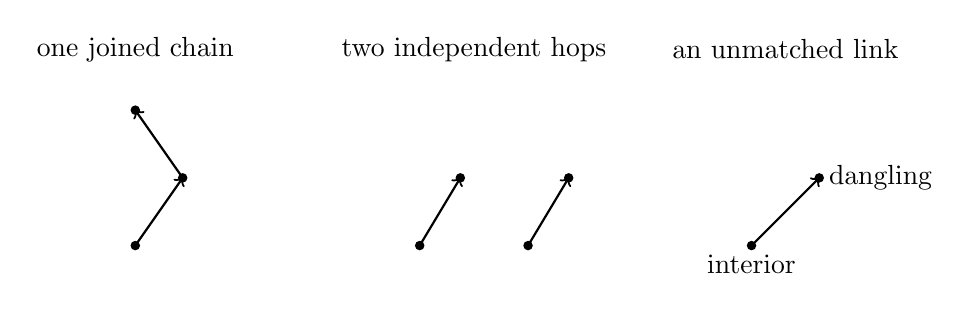
\begin{tikzpicture}[scale=0.86]
\node at (0,2.9) {one joined chain};
\fill (0,0) circle (2pt);
\fill (0.7,1.0) circle (2pt);
\fill (0,2.0) circle (2pt);
\draw[thick,->] (0,0) -- (0.7,1.0);
\draw[thick,->] (0.7,1.0) -- (0,2.0);

\begin{scope}[xshift=4.2cm]
\node at (0.8,2.9) {two independent hops};
\fill (0,0) circle (2pt);
\fill (0.6,1.0) circle (2pt);
\fill (1.6,0) circle (2pt);
\fill (2.2,1.0) circle (2pt);
\draw[thick,->] (0,0) -- (0.6,1.0);
\draw[thick,->] (1.6,0) -- (2.2,1.0);
\end{scope}

\begin{scope}[xshift=9.1cm]
\node at (0.5,2.9) {an unmatched link};
\fill (0,0) circle (2pt);
\fill (1.0,1.0) circle (2pt);
\draw[thick,->] (0,0) -- (1.0,1.0);
\node[below] at (0,0) {interior};
\node[right] at (1.0,1.0) {dangling};
\end{scope}
\end{tikzpicture}%
}
\caption{اختيارات موصولة، ومستقلة، وغير مقترنة، لوصلات متجاورة.}
\end{figure}

قد يوجد بالفعل أكثر من مسار واحد عند هذه الرتبة. فبالنسبة إلى إزاحة بمقدار خطوة شبكية زمنية واحدة وخطوة مكانية واحدة، يصل التسلسلان
\begin{align}
x
&\longrightarrow x+\hat t
\longrightarrow x+\hat t+\hat s,\\
x
&\longrightarrow x+\hat s
\longrightarrow x+\hat s+\hat t
\end{align}
إلى نقطة النهاية نفسها.

\begin{classroomqa}
\lecturetimestamp{00:55:53}
\audiencequestion{هل يوجد مسار آخر من خطوتين إلى نقطة النهاية القطرية نفسها؟}
\lecturerresponse{نعم. يمكن أخذ الخطوة الزمنية أولًا ثم الخطوة المكانية ثانيًا، أو أخذهما بالترتيب المعاكس. وكلا المسارين يسهم في سعة الانتقال نفسها.}
\end{classroomqa}

ولا يوجد ما يدعو إلى التوقف عند وصلتين. فالحد من الرتبة الثالثة يوفّر سلاسل من ثلاث وصلات متجاورة. وقد يتقدّم مسار ما مباشرة، أو يقوم بالتفاف، أو يبتعد ثم يعود قبل بلوغ النقطة النهائية. وتشمل الرتب الأعلى من ذلك التفافات أطول ورجوعًا متكررًا على الأثر. ولذلك فإن التوسيع إلى رتبة اعتباطية يولّد إسهامًا لكل مسار مركّب من وصلات محلية. والسعة من نقطة إلى نقطة هي مجموعها كلها، بمعاملات تحتوي القوى المناسبة لـ \(i\) وعوامل المضروب:
\begin{equation}
\begin{gathered}
\mathcal{A}(x_{\mathrm{in}}\to x_{\mathrm{out}})
=
\sum_{\text{joined lattice routes }r}c_r,
\\
c_r\ \hbox{read from the exponential expansion}.
\end{gathered}
\end{equation}
والمعاملات، بوجه عام، عقدية، لذا تكون السعة الناتجة عقدية.

يضيف الانتشار النسبي إمكانية أخرى. فقد يسير مسار ما صعودًا وهبوطًا في اتجاه الزمن، وقد يعبر الوصلة نفسها مرارًا.

\begin{classroomqa}
\lecturetimestamp{00:58:47}
\audiencequestion{هل يمكن لمسار أن يمر عبر الخليتين نفسيهما مرارًا وتكرارًا؟}
\lecturerresponse{نعم. تُحتسب الاجتيازات المتكررة، وفي التوسع النسبي قد يسير المسار أيضًا إلى الخلف في الزمن.}
\end{classroomqa}

يتيح مقطع راجع في الزمن قراءتين رسوميتين متكافئتين. فيمكن التعامل معه بوصفه خط جسيم يسير إلى الخلف في الزمن. وبدلًا من ذلك، إذا تتبعنا الزمن إلى الأمام فقط، فإن زوجًا جسيم--ضديد الجسيم يُستحدث، ويواصل الجسيم منه سيره إلى الأمام، ثم يلتقي ضديد الجسيم لاحقًا بالجسيم الأصلي ويفنيه. والخط المتصل نفسه يشفّر كلا الوصفين.\footnote{تتبع القراءتان الرسم والشرح عند 00:59:00--00:59:51.}

\begin{figure}[htbp]
\centering
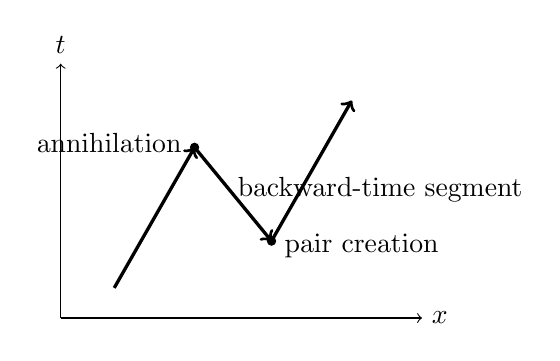
\begin{tikzpicture}[scale=0.85]
\draw[->] (0,0) -- (0,3.8) node[above] {$t$};
\draw[->] (0,0) -- (5.4,0) node[right] {$x$};
\draw[very thick,->] (0.8,0.45) -- (2.0,2.55);
\draw[very thick,->] (2.0,2.55) -- (3.15,1.15);
\draw[very thick,->] (3.15,1.15) -- (4.35,3.25);
\fill (2.0,2.55) circle (2pt);
\fill (3.15,1.15) circle (2pt);
\node[left] at (1.95,2.62) {annihilation};
\node[right] at (3.20,1.08) {pair creation};
\node[right] at (2.50,1.92) {backward-time segment};
\end{tikzpicture}
\caption{مقطع راجع في الزمن يُقرأ إلى الأمام بوصفه استحداث زوج وإفناءه.}
\end{figure}

تضبط عوامل المضروب التي تظهر عند الرتب العالية متسلسلة الأس، لكن ذلك ليس هو نفسه ضبط المجموع الكامل على تشكيلات الحقول.

\begin{classroomqa}
\lecturetimestamp{01:00:00}
\audiencequestion{هل تضمن عوامل \(1/n!\) التقارب؟}
\lecturerresponse{هي تضمن تقارب متسلسلة الأس لحجة ثابتة. لكنها لا تضمن بذاتها تقارب المجموع المنفصل على جميع تشكيلات الحقول. وهذان سؤالان متميزان. وعلى شبكة منتهية ذات مجموعة متقطعة منتهية من قيم الحقل، يكون عدد التشكيلات منتهيًا، لكن حدي الاستمرار والحجم اللانهائي يتطلبان ضبطًا إضافيًا.}
\end{classroomqa}

\section{جداء وصلة واحدة وقراءات جسيمية متعددة}

يحتوي جداء الرتبة الثانية على أكثر من مجرد انتشار أحادي الجسيم. فعندما يشترك زوجاه المتجاوران في نقطة نهاية، يمكنه أن ينقل جسيمًا واحدًا عبر سلسلة من وصلتين:
\begin{equation}
\bigl[\phi(x_0)\phi(x_1)\bigr]
\bigl[\phi(x_1)\phi(x_2)\bigr].
\end{equation}
وعندما يكون الزوجان المختاران منفصلين، يمكن للحد نفسه من الرتبة الثانية أن ينقل جسيمين، كلًّا منهما عبر وصلة واحدة.\footnote{أُعيد بناء المقارنة بين الانتشار أحادي الجسيم وقفزتين مستقلتين أحاديتَي الوصلة من مناقشة اللوح عند 01:00:46--01:02:34.}
\begin{equation}
\bigl[\phi(x_0)\phi(x_1)\bigr]
\bigl[\phi(y_0)\phi(y_1)\bigr],
\qquad x_0\neq y_0.
\end{equation}
ينقل العامل الأول جسيمًا، وينقل الثاني جسيمًا آخر. وهكذا يحتوي التوسع الشبكي التربيعي على سعات انتشار في كل قطاع متعدد الجسيمات. وقد تصف الرتبة الجبرية نفسها مسارًا متصلًا أطول واحدًا أو عدة مسارات أقصر غير متصلة.

هذا قدر كبير من المعلومات، لكنه ليس بعدُ رأس تفاعل حقيقيًا. فمع وجود حدود انتشار تربيعية فقط، لا تنشطر خطوط الجسيمات المتصلة إلى عدد مختلف من الخطوط. وتتطلب العمليات التي تغيّر عدد الجسيمات تفاعلات إضافية، حتى وإن كانت جداءات المؤثرات الموضعية قد تتيح عدة قراءات على هيئة استحداث وإفناء.

\begin{classroomqa}
\lecturetimestamp{01:03:30}
\audiencequestion{هل يمكن لإلكترون وبوزيترون أن يفنيا ولا يتركا أي جسيمات على الإطلاق؟}
\lecturerresponse{إن إسهامًا ذا طاقة داخلة غير منعدمة ومن دون حالة نهائية حاملة للطاقة ينتهك انحفاظ الطاقة. وعند الجمع على مواضعه الزمكانية الممكنة، تتلاشى السعات. ويمكن أن يحدث إفناء إلكترون--بوزيترون عندما يحمل حقل آخر الطاقة بعيدًا---على سبيل المثال، عندما تُنتَج كمّات كهرومغناطيسية.}
\end{classroomqa}

\editorialnote{ينتقل هذا التبادل المقتضب مباشرةً من القفز التربيعي إلى إفناء إلكترون--بوزيترون. والتمييز الموثوق هو أن الحدود التربيعية تؤمّن الانتشار الحر، في حين أن الإفناء الفيزيائي يتطلب تفاعلًا مع حقل آخر؛ أما السعة عديمة المخرجات فتتلاشى بسبب حفظ الطاقة.}

تنجز حدود المشتقات إذن كثيرًا من العمل، لكنها لا تنجز كل شيء. وتتحدد حدود أخرى في اللاغرانجيان بخصائص الحقول وتفاعلاتها المرصودة تجريبيًا.

\section{حد الكتلة}

بالنسبة إلى حقل قياسي، فإن بنية المشتقات قيد المناقشة لها نمط إشارات لورنتزي تخطيطي
\begin{equation}
\mathcal{L}_{\mathrm{kin}}
\sim
\frac{1}{2}\left[
(\partial_t\phi)^2
-(\partial_x\phi)^2
-(\partial_y\phi)^2
-(\partial_z\phi)^2
\right].
\end{equation}
ويثبت هذا العرض بنية الزمن ناقص المكان ذات الصلة بالمناقشة؛ وتُترك اتفاقيات الإشارة الكلية والتطبيع ضمنية.

قد يحتوي اللاغرانجيان أيضًا على قوى الحقل غير المشتق. ويأخذ المثال التربيعي الصورة
\begin{equation}
\text{mass term}\ \propto\ \frac{1}{2}m^2\phi^2,
\end{equation}
حيث يُعرَّف \(m^2\) بوصفه معامل الكتلة.\editorialnote{لا يثبت المصدر في هذا الموضع اتفاقية الإشارة الكلية للاغرانجيان القياسي الكامل.} وفي القراءة الجسيمية التخطيطية، يفني هذا الحد جسيمًا ويعيد خلقه في الموقع الشبكي نفسه. وهو لا يزيح الجسيم. بل يُدرج عاملًا في الموضع نفسه داخل مسار:
\begin{equation}
\text{particle at }x
\longrightarrow
\boxed{m^2\phi(x)^2}
\longrightarrow
\text{particle still at }x.
\end{equation}
وكلما أثّر إدراج من هذا القبيل، اكتسب المسار عاملًا إضافيًا متناسبًا مع \(m^2\).

إذا أبقينا على حدود المشتقات وحدها، فإن الانتشار الناتج في هذا التوسع التخطيطي هو انتشار النظرية عديمة الكتلة. أما بالنسبة إلى حقل ذي كتلة، فقد يشتمل مسار ما على أي عدد من إدراجات الكتلة في الموضع نفسه بين حدود قفزه. ويغيّر حد الكتلة الأوزان النسبية للمسارات بحيث يحمل المنتشر الناتج كتلة الجسيم.

\section{الحدود التكعيبية وتواريخ الانقسام--إعادة الالتحام}

يغيّر حد الكتلة وزن المسار من دون أن يحرّك الجسيم. ويبدأ سلوك أكثر إثارة مع الحدود الأعلى من الدرجة الثانية. خذ تفاعلًا تكعيبيًا،
\begin{equation}
\mathcal{L}_{\mathrm{int}}=g_3\phi^3.
\end{equation}
في خلية شبكية واحدة، تكون لعوامل الحقل الثلاثة أربع قراءات جسيمية:
\begin{equation}
1\longrightarrow 2,
\qquad
2\longrightarrow 1,
\qquad
0\longrightarrow 3,
\qquad
3\longrightarrow 0.
\end{equation}
وعليه، قد يفني عامل تكعيبي جسيمًا واحدًا ويخلق جسيمين، أو يفني جسيمين ويخلق جسيمًا واحدًا، أو يخلق ثلاثة جسيمات، أو يفني ثلاثة جسيمات.

لا تزال عوامل الأزواج المتجاورة التربيعية تؤمّن الانتشار. ويمكن لتتابع منها أن يحمل جسيمًا إلى خلية، ويمكن لعامل تكعيبي في تلك الخلية أن يمتصه ويصدر جسيمين، ويمكن لعوامل تربيعية أخرى أن تحمل هذين الجسيمين بعيدًا. وهذا يسهم في سعة لها جسيم وارد واحد وجسيمان صادران.\footnote{تُعاد هندسة الشبكة بناؤها من الشكل عند 01:08:48--01:09:42.}

\begin{figure}[htbp]
\centering
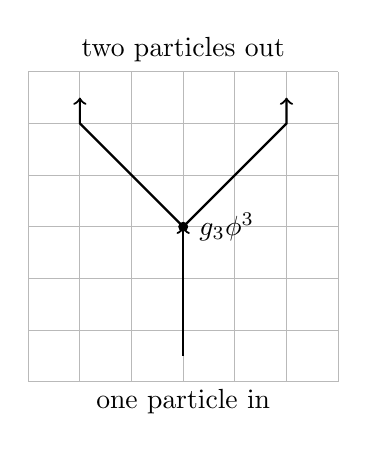
\begin{tikzpicture}[scale=0.82]
\draw[step=0.8,gray!55,thin] (0,0) grid (4.8,4.8);
\draw[thick,->] (2.4,0.4) -- (2.4,1.2) -- (2.4,2.0) -- (2.4,2.4);
\fill (2.4,2.4) circle (2.2pt);
\draw[thick,->] (2.4,2.4) -- (1.6,3.2) -- (0.8,4.0) -- (0.8,4.4);
\draw[thick,->] (2.4,2.4) -- (3.2,3.2) -- (4.0,4.0) -- (4.0,4.4);
\node[right] at (2.5,2.4) {$g_3\phi^3$};
\node at (2.4,-0.3) {one particle in};
\node at (2.4,5.15) {two particles out};
\end{tikzpicture}
\caption{تحمل العوامل التربيعية جسيمًا إلى رأس انقسام تكعيبي ثم بعيدًا عنه.}
\end{figure}

حتى السعة التي يكون فيها جسيم واحد في البداية وفي النهاية لم تعد مجرد مجموع لمسارات مفردة غير منقطعة. إحدى المساهمات هي الانتشار المباشر عبر سلسلة من القفزات التربيعية. ومساهمة أخرى تحتوي على عاملين تكعيبيين: ينقسم الجسيم إلى اثنين ثم يلتحم الاثنان من جديد لاحقًا. ولذلك قد تحتوي الحالة الوسيطة على جسيمات أكثر من الحالة الخارجية.\footnote{يُعاد بناء البديلين من الشكل عند 01:09:44--01:11:36.}

\begin{figure}[htbp]
\centering
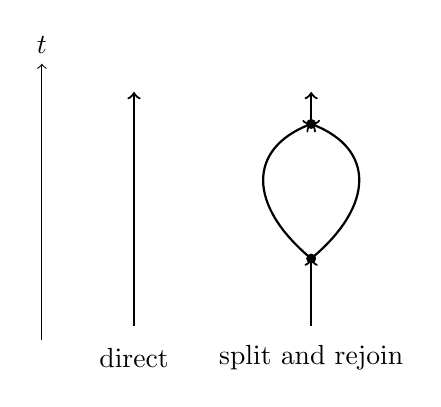
\begin{tikzpicture}[scale=0.9]
\draw[->] (-0.7,0) -- (-0.7,3.9) node[above] {$t$};
\draw[thick,->] (0.6,0.2) -- (0.6,3.5);
\node at (0.6,-0.25) {direct};
\draw[thick,->] (3.1,0.2) -- (3.1,1.15);
\fill (3.1,1.15) circle (2pt);
\draw[thick,->] (3.1,1.15) .. controls (2.2,1.9) and (2.2,2.7) .. (3.1,3.05);
\draw[thick,->] (3.1,1.15) .. controls (4.0,1.9) and (4.0,2.7) .. (3.1,3.05);
\fill (3.1,3.05) circle (2pt);
\draw[thick,->] (3.1,3.05) -- (3.1,3.5);
\node at (3.1,-0.25) {split and rejoin};
\end{tikzpicture}
\caption{الانتشار المباشر ومساهمة انقسام--التحام من جديد في سعة الجسيم الواحد نفسها.}
\end{figure}

في الكهروديناميكا، المثال المناظر هو إلكترون يصدر فوتونًا ثم يعيد امتصاصه لاحقًا. وذلك التاريخ القائم على الإصدار ثم إعادة الامتصاص هو جزء من السعة لانتشار الإلكترون من نقطة إلى أخرى. وتتضمن الرتب الأعلى عدة عمليات إصدار وامتصاص. وقد يتحول الفوتون إلى زوج إلكترون--بوزيترون، وقد يتبادل الإلكترون والبوزيترون في ذلك الزوج الوسيط فوتونًا بينهما. ولا شيء يوجب أن يكون محتوى الجسيمات الوسيط بسيطًا لمجرد أن محتوى الجسيمات الابتدائي والنهائي بسيط.\footnote{تَرِد الأمثلة في إعادة البناء التالية عند 01:11:22--01:12:34.}

\begin{figure}[htbp]
\centering
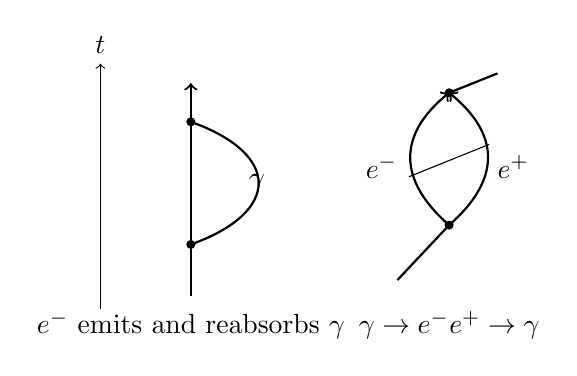
\begin{tikzpicture}[scale=0.82]
\draw[->] (-0.6,0) -- (-0.6,3.8) node[above] {$t$};
\draw[thick,->] (0.8,0.2) -- (0.8,3.5);
\fill (0.8,1.0) circle (2pt);
\fill (0.8,2.9) circle (2pt);
\draw[thick] (0.8,1.0) .. controls (2.2,1.5) and (2.2,2.4) .. (0.8,2.9);
\node[right] at (1.55,1.95) {$\gamma$};
\node at (0.8,-0.25) {$e^-$ emits and reabsorbs $\gamma$};
\draw[thick] (4.0,0.45) -- (4.8,1.3);
\fill (4.8,1.3) circle (2pt);
\draw[thick,->] (4.8,1.3) .. controls (4.0,2.0) and (4.0,2.7) .. (4.8,3.35);
\draw[thick,->] (4.8,1.3) .. controls (5.6,2.0) and (5.6,2.7) .. (4.8,3.35);
\fill (4.8,3.35) circle (2pt);
\draw[thick] (4.8,3.35) -- (5.55,3.65);
\draw[thin] (4.18,2.05) -- (5.42,2.55);
\node[left] at (4.15,2.2) {$e^-$};
\node[right] at (5.4,2.2) {$e^+$};
\node at (4.8,-0.25) {$\gamma\to e^-e^+\to\gamma$};
\end{tikzpicture}
\caption{مساهمة انبعاث ذاتي لإلكترون، وتاريخ لفوتون يحتوي على زوج إلكترون--بوزيترون.}
\end{figure}

ينشأ كل تاريخ من هذا النوع من جداء محدد لحدود في توسع الأسي. ويحمل معامله القوة المناسبة لـ \(i\)، وعاملًا عامليًا من متسلسلة الأسي، والاقترانات المرتبطة برؤوسه. ويعطي المعامل مساهمة ذلك التاريخ، لكن السعة للحالتين الابتدائية والنهائية المحددتين هي مجموع جميع التواريخ التي لها تلك الحالات الخارجية نفسها.

\begin{classroomqa}
\lecturetimestamp{01:13:18}
\audiencequestion{هل يمكن أن تتحقق العملية الكلية نفسها عبر عدة تواريخ مختلفة بحيث تسهم كلها في سعتها؟}
\lecturerresponse{نعم. تُستخرج سعة العملية من جميع التواريخ المختلفة التي تصل الحالة الابتدائية نفسها بالحالة النهائية نفسها.}
\end{classroomqa}

وعليه، توجد طريقتان متكافئتان لصياغة نظرية الحقل الكمومي. ففي الوصف الحقلي، نحدد تشكيلًا حقليًا ابتدائيًا وتشكيلًا حقليًا نهائيًا ونجمع على كل تاريخ حقلي متدخل بينهما. وفي الوصف الجسيمي، يُحلَّل الحقل إلى كمّات: نحدد محتوى الجسيمات الواردة ومحتوى الجسيمات الصادرة ونجمع جميع التواريخ الجسيمية التي تصل بينهما. ويحكم اللاغرانجيان نفسه كلا الوصفين.

\section{الحدود الرباعية، وقوانين الانحفاظ، والاقترانات}

تفاعل رباعي،
\begin{equation}
\mathcal{L}_{\mathrm{int}}=g_4\phi^4,
\end{equation}
له أربعة عوامل حقل في نقطة واحدة. وتشمل قراءاته الجسيمية الموضعية
\begin{equation}
\begin{gathered}
2\longrightarrow2,
\qquad
1\longrightarrow3,
\qquad
3\longrightarrow1,\\
0\longrightarrow4,
\qquad
4\longrightarrow0.
\end{gathered}
\end{equation}
ولذلك يمكن لرأس واحد ذي أربع أرجل أن يصف تبعثر جسيمين، أو انقسام جسيم واحد إلى ثلاثة، أو التحام ثلاثة في واحد، أو كون الأرجل الأربع كلها موجهة إلى الخارج أو إلى الداخل.\footnote{تُستعاد هذه الاتجاهات من الشكل عند 01:14:28--01:15:18.}

\begin{figure}[htbp]
\centering
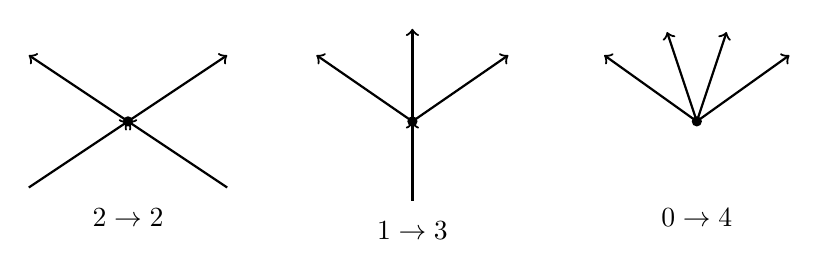
\begin{tikzpicture}[scale=0.84]
\fill (0,0) circle (2.2pt);
\draw[thick,->] (-1.5,-1.0) -- (0,0);
\draw[thick,->] (1.5,-1.0) -- (0,0);
\draw[thick,->] (0,0) -- (-1.5,1.0);
\draw[thick,->] (0,0) -- (1.5,1.0);
\node at (0,-1.45) {$2\to2$};
\begin{scope}[xshift=4.3cm]
\fill (0,0) circle (2.2pt);
\draw[thick,->] (0,-1.2) -- (0,0);
\draw[thick,->] (0,0) -- (-1.45,1.0);
\draw[thick,->] (0,0) -- (0,1.4);
\draw[thick,->] (0,0) -- (1.45,1.0);
\node at (0,-1.65) {$1\to3$};
\end{scope}
\begin{scope}[xshift=8.6cm]
\fill (0,0) circle (2.2pt);
\draw[thick,->] (0,0) -- (-1.4,1.0);
\draw[thick,->] (0,0) -- (-0.45,1.35);
\draw[thick,->] (0,0) -- (0.45,1.35);
\draw[thick,->] (0,0) -- (1.4,1.0);
\node at (0,-1.45) {$0\to4$};
\end{scope}
\end{tikzpicture}
\caption{ثلاثة اتجاهات موضعية لرأس تفاعل ذي أربع أرجل.}
\end{figure}

القراءة الموضعية \(0\to4\) لا تعني بذاتها أن أربعة جسيمات يمكن أن تظهر من الفراغ بوصف ذلك عملية فيزيائية. فلا بد مع ذلك من الجمع على جميع المواضع الزمكانية الممكنة للرأس. وعندما لا يمكن للحالة الخارجية المقترحة أن تحقق حفظ الطاقة، تتلاشى الأطوار الآتية من تلك المواضع بعضها مع بعض.

\begin{classroomqa}
\lecturetimestamp{01:15:18}
\audiencequestion{هل يصف الاتجاه ذو الأرجل الأربع إلى الخارج الوصول التلقائي لأربعة جسيمات في الحالة النهائية؟}
\lecturerresponse{إنه قراءة موضعية واحدة لمؤثر الحقول الأربعة، لكن عمليةً من دون طاقة داخلة تنتهك حفظ الطاقة. وعندما تُجمع السعات من جميع المواضع الزمكانية الممكنة للرأس، تتلاشى إلى الصفر.}
\end{classroomqa}

\begin{classroomqa}
\lecturetimestamp{01:15:58}
\audiencequestion{هل ينبثق حفظ الطاقة وحفظ الزخم من الحساب نفسه؟}
\lecturerresponse{نعم. إن تكامل الرأس على جميع الأزمنة يفرض حفظ الطاقة، وتكامله على جميع أنحاء الفضاء يفرض حفظ الزخم. ويزول المجموع على مواضع الرأس إلا إذا حُفظا معًا.}
\end{classroomqa}

مع مراعاة قوانين الانحفاظ تلك، يسهم كل مخطط يسمح به اللاغرانجيان في سعة ما. ويتوقف مقدار تلك المساهمة جزئيًا على معامل كل حد تفاعل. ولنكتب معاملي الحدين التكعيبي والرباعي على أنهما \(G_3\) و\(G_4\). ويسهم كل رأس ذي ثلاث أرجل بعامل واحد من \(G_3\)، ويسهم كل رأس ذي أربع أرجل بعامل واحد من \(G_4\). ولذلك يكون لمخطط يحوي \(V_3\) رؤوسًا تكعيبية و\(V_4\) رؤوسًا رباعية الاعتماد التخطيطي التالي على الاقترانات
\begin{equation}
\mathcal{A}_{\mathrm{graph}}
\propto G_3^{V_3}G_4^{V_4}.
\end{equation}

إذا كانت هذه الاقترانات صغيرة، فإن مخططًا ذا رؤوس قليلة يسهم عادةً أكثر من مخطط ذي رؤوس كثيرة. فكل رأس إضافي يجلب عاملًا صغيرًا آخر. وهذا يمنح المجموع الاضطرابي فرصة لأن يكون مفيدًا: نبدأ بأبسط المخططات، ثم نضيف تصحيحات أصغر فأصغر تباعًا.

وسؤال ما إذا كانت السلسلة الكاملة تتقارب فعلًا سؤال صعب. فالاقترانات الصغيرة تجعل هذا الترتيب معقولًا، لكنها لا تحسم بمفردها كل مشكلة من مشكلات التقارب. وعند الاقتران الكبير قد تفشل السلسلة الساذجة بالكامل. ولا يدل مثل هذا الفشل على أن النظرية الكامنة خاطئة؛ بل قد يدل فقط على أن التوسع في قوى الاقتران كان طريقة غير جيدة لحسابها. وتكون الطرائق قيد المناقشة أنفع ما تكون مباشرةً عندما تكون الاقترانات صغيرة بما يكفي بحيث يكون مخطط ذو أربعة رؤوس أصغر بكثير من مخطط ذي رأسين.

\begin{classroomqa}
\lecturetimestamp{01:19:24}
\audiencequestion{هل يمكن معالجة نظرية اللون بالطريقة نفسها؟}
\lecturerresponse{نعم. يمكن صياغة نظرية اللون بالطريقة نفسها، وستناقش لاحقًا.}
\end{classroomqa}

\section{مؤثرات الانتشار، والرؤوس، والأوصاف المتتامة}

المهمة التالية هي تعداد الجسيمات وترميز دينامياتها إما في لاغرانجيان أو في قواعد فاينمان. وهذان شكلان للمعلومة نفسها. تصف الحدود التربيعية الانتشار من نقطة إلى أخرى. ويُسمّى الخط الذي يمثّل ذلك الانتشار مؤثر انتشار. أما الحدود التي تتضمن ثلاثة حقول أو أكثر فتصف المواضع التي تلتقي فيها الخطوط. ونقاط الالتقاء تلك هي الرؤوس. على سبيل المثال،
\begin{equation}
\begin{aligned}
\text{quadratic term}
&\longleftrightarrow \text{propagator},\\
G_3\phi^3
&\longleftrightarrow \text{three-leg vertex}.
\end{aligned}
\end{equation}

يمكن تحديد نظرية بإعطاء حقل كمومي لكل جسيم وكتابة لاغرانجيان واحد يحتوي جميع كتلها وتفاعلاتها. وبصورة مكافئة، يمكن سرد كل مؤثر انتشار، وكل رأس مسموح به، والمعامل المرتبط بكل رأس. وأيٌّ من القائمتين يخبرنا ما العمليات الممكنة وكيف نُسند السعات إلى مخططاتها.

فعلى سبيل المثال، يمكن لإلكترونين أن يتشتتا بتبادل فوتون. ويحتوي كل خط إلكترون على رأس إلكترون--إلكترون--فوتون، ويصل مؤثر انتشار الفوتون بين الرأسين.\footnote{أُعيد بناء المخطط انطلاقًا من المثال عند 01:21:38.}

\begin{figure}[htbp]
\centering
\begin{tikzpicture}[scale=0.95]
\draw[->] (-0.6,-0.2) -- (0.2,1.4);
\draw[->] (0.2,1.4) -- (-0.7,3.1);
\draw[->] (3.5,-0.2) -- (2.7,1.4);
\draw[->] (2.7,1.4) -- (3.6,3.1);
\fill (0.2,1.4) circle (2pt);
\fill (2.7,1.4) circle (2pt);
\draw[thick] (0.2,1.4) -- (2.7,1.4);
\node[above] at (1.45,1.4) {$\gamma$};
\node[left] at (-0.2,0.5) {$e^-$};
\node[right] at (3.1,0.5) {$e^-$};
\end{tikzpicture}
\caption{تشتت إلكترونين عبر تبادل فوتون.}
\end{figure}

يحدّد اللاغرانجيان السعة لهذا المخطط، ويحتوي التناظرات وقوانين الانحفاظ التي تقيّده. وفي رسم موجَّه زمنيًا، تشكّل الجسيمات الموضوعة في الأسفل التهيئة الابتدائية، وتشكل الجسيمات في الأعلى التهيئة النهائية.

\begin{classroomqa}
\lecturetimestamp{01:22:06}
\audiencequestion{في مخطط فاينمان، هل تكون الجسيمات في الأسفل هي التهيئة الابتدائية وتكون تلك في الأعلى هي التهيئة النهائية؟}
\lecturerresponse{نعم. فالأسفل هو تهيئة الجسيمات الابتدائية، والأعلى هو تهيئة الجسيمات النهائية.}
\end{classroomqa}

وصف الجسيمات ووصف الحقول متتامان، تمامًا كما أن الزخم والموضع وصفان متتامان في ميكانيكا الكم الاعتيادية. فهما يصفان النظام نفسه في أساسين مختلفين. وهناك أيضًا لايقين مناظر: إذا حُدِّد عدد الجسيمات بدقة فإن قيمة الحقل تكون غير يقينية؛ وإذا حُدِّدت قيمة الحقل بدقة فإن عدد الجسيمات يكون غير يقيني. ولا يحل أيٌّ من الوصفين محلَّ الآخر، واللاغرانجيان مفيد في كليهما.

\begin{classroomqa}
\lecturetimestamp{01:23:26}
\audiencequestion{هل تتنبأ النظرية بثوابت الاقتران، أم تُحدَّد تجريبيًا؟}
\lecturerresponse{يمكن للتناظرات أحيانًا أن تربط ثابت اقتران بآخر، لكن قيمها العددية تأتي عمومًا من التجربة.}
\end{classroomqa}

\section{المدخلات المقاسة والتنبؤات الواسعة}

إن نظرية الحقل الكمومي نفسها تتسم بالأناقة والجمال. ولكن حين يبدأ المرء في تعداد الحقائق---ما الجسيمات الموجودة، وما كتلها، وما ثوابت اقترانها---تبدو القائمة فوضوية. إنها فوضى شديدة القبح، وبها قدر ضئيل جدًا من الاتساق، باستثناء الاتساق الذي توفره التناظرات. فالتناظرات تربط بين الأنواع المختلفة من الجسيمات وعملياتها، ولكن إلى حد محدود فقط. ويبقى جزء كبير من هذا الجرد مجرد مجموعة كبيرة من الحقائق العشوائية نسبيًا عن مجموعة من الأنواع المختلفة من الجسيمات لا يبدو أن وراءها دافعًا واضحًا كثيرًا.

\begin{classroomqa}
\lecturetimestamp{01:24:58}
\audiencequestion{لماذا ينبغي الوثوق بثوابت الاقتران المقاسة بهذه الثقة الكبيرة؟}
\lecturerresponse{ما إن يُقاس اقتران حتى يؤدّي تغييره إلى تنبؤات غير صحيحة. وتُختبَر قيمته من خلال الحسابات الكثيرة التي تستخدمه.}
\end{classroomqa}

هناك جسيمات كثيرة جدًا، ما يعني حقولًا كثيرة جدًا---أكثر مما يطيقه أي حس جمالي. وعددها يقارب المئة أو نحو ذلك. وهناك كثير من ثوابت الاقتران، وهي إلى حد ما أعداد مأخوذة من التجربة، وكثير من الكتل التي تتفاوت تفاوتًا هائلًا. وتوجد فيما بينها علاقات قليلة، ولكنها قليلة فحسب.

لكن ما إن تعرفها حتى يمكنك أن تبدأ الحساب. وما إن تعرفها فذلك كل ما يلزم: يمكن للمرء أن يحسب بدقة كبيرة أي شيء يتعلق بتلك الجسيمات. وكل ما يتعلق بالكواركات والإلكترونات والفوتونات وسائرها يمتد إلى الفيزياء الذرية، وفيزياء الجسيمات، والفيزياء النووية، والكيمياء، وربما الأحياء. قد يكون مقدار المدخلات أكبر مما يود المرء، لكن مقدار المخرجات هائل.

\section{الديناميكا الكهربائية الكمومية كمثال اضطرابي}

تقدّم الديناميكا الكهربائية الكمومية مثالًا ملموسًا على توسّع الاقتران.

\begin{classroomqa}
\lecturetimestamp{01:26:12}
\audiencequestion{بالنسبة إلى الإلكترونات والفوتونات، كم عدد اقترانات التفاعل من نوع \(G_n\)؟}
\lecturerresponse{يوجد اقتران تفاعل أولي واحد: الشحنة الكهربائية \(e\). وهو معامل من نوع \(G_3\) مرتبط برأس يدخل فيه إلكترون ويخرج منه إلكترون ويُبعث فيه فوتون أو يُمتص.}
\end{classroomqa}

مع إهمال المصفوفات السبينورية والفهارس، يكون للتفاعل المحتوى الحقلي التخطيطي الآتي
\begin{equation}
\mathcal{L}_{\mathrm{QED,int}}
\sim e\,(\text{electron bilinear})\,A,
\end{equation}
حيث إن \(A\) يدل على حقل الفوتون. ولا نحتاج إلى البنية التفصيلية لمصفوفات ديراك في حجة العدّ. والقاعدة الأولية في الديناميكا الكهربائية الكمومية هي أن يصدر الإلكترون فوتونًا أو يمتصه؛ وجميع مخططات الديناميكا الكهربائية الكمومية الأكثر تعقيدًا تُركَّب من الاستعمال المتكرر لذلك الرأس الواحد.\footnote{أُعيد بناء الرأس التخطيطي من 01:26:42؛ وقد حُجبت عمدًا في الأصل البنية المصفوفية التفصيلية.}

\begin{figure}[htbp]
\centering
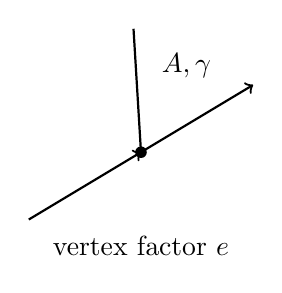
\begin{tikzpicture}[scale=0.95]
\draw[thick,->] (-1.5,-0.9) -- (0,0);
\draw[thick,->] (0,0) -- (1.5,0.9);
\draw[thick] (0,0) -- (-0.1,1.65);
\fill (0,0) circle (2.2pt);
\node[right] at (0.15,1.15) {$A,\gamma$};
\node at (0,-1.25) {vertex factor $e$};
\end{tikzpicture}
\caption{الرأس الأولي إلكترون--إلكترون--فوتون في الديناميكا الكهربائية الكمومية.}
\end{figure}

\begin{classroomqa}
\lecturetimestamp{01:27:38}
\audiencequestion{وماذا عن تشتت إلكترون--بروتون؟}
\lecturerresponse{في المعالجة الذرية الأولية، يمكن تمثيل البروتون على نحو مثالي بوصفه مصدرًا نقطيًا ثابتًا ذا كتلة لا نهائية---جسيمًا ثقيلًا مُثبَّتًا في مكانه. ولا تدخل دينامياته الحقلية الكمومية الخاصة إلا عندما تُدرج النظرية الداخلية للبروتونات والنيوترونات.}
\end{classroomqa}

\begin{classroomqa}
\lecturetimestamp{01:28:30}
\audiencequestion{هل يمكن للإلكترون أن يتحرك بسرعة تقارب سرعة الضوء بالنسبة إلى ذلك البروتون؟}
\lecturerresponse{نعم.}
\end{classroomqa}

لننظر في تشتت فوتون على إلكترون. عند الرتبة الدنيا يكون في المخطط رأسان إلكترون--إلكترون--فوتون. ولذلك تكون السعة متناسبة مع \(e^2\):
\begin{equation}
\mathcal{A}_{\mathrm{lowest}}\propto e^2.
\end{equation}
أما الاحتمال، أو بصورة مكافئة اعتماد المقطع العرضي على الاقتران، فيأتي من مربع القيمة المطلقة ويكون متناسبًا مع \(e^4\):
\begin{equation}
P_{\mathrm{lowest}}\ \text{or}\ \sigma_{\mathrm{lowest}}
\propto e^4.
\end{equation}
ومع التطبيع اللابعدي المألوف، يكون الاقتران الكهربائي صغيرًا، لذا فإن حدوث تشتت فعلي أقل احتمالًا بكثير من أن يمر الفوتون ببساطة من دون تشتت.

يوجد بالفعل مخططان عند هذه الرتبة. ففي أحد الترتيبين يُمتص الفوتون الوارد ثم يُصدَر الفوتون الصادر لاحقًا. وفي الآخر يُصدَر الفوتون الصادر قبل أن يُمتص الفوتون الوارد. وكلتا السعتين تسهمان.\footnote{أُعيد بناء الترتيبين الزمنيين من المخططين عند 01:28:42 و01:30:18.}

\begin{figure}[htbp]
\centering
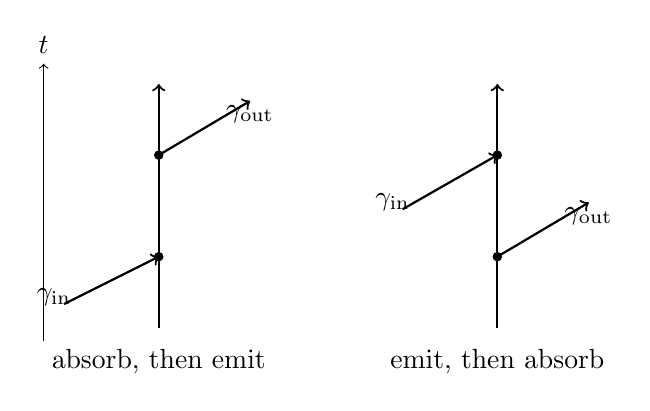
\begin{tikzpicture}[scale=0.86]
\draw[->] (-0.7,0) -- (-0.7,4.1) node[above] {$t$};
\draw[thick,->] (1.0,0.2) -- (1.0,3.8);
\fill (1.0,1.25) circle (2pt);
\fill (1.0,2.75) circle (2pt);
\draw[thick,->] (-0.4,0.55) -- (1.0,1.25);
\draw[thick,->] (1.0,2.75) -- (2.35,3.55);
\node[left] at (-0.15,0.65) {$\gamma_{\mathrm{in}}$};
\node[right] at (1.85,3.35) {$\gamma_{\mathrm{out}}$};
\node at (1.0,-0.3) {absorb, then emit};
\begin{scope}[xshift=5.0cm]
\draw[thick,->] (1.0,0.2) -- (1.0,3.8);
\fill (1.0,1.25) circle (2pt);
\fill (1.0,2.75) circle (2pt);
\draw[thick,->] (1.0,1.25) -- (2.35,2.05);
\draw[thick,->] (-0.4,1.95) -- (1.0,2.75);
\node[right] at (1.85,1.85) {$\gamma_{\mathrm{out}}$};
\node[left] at (-0.15,2.05) {$\gamma_{\mathrm{in}}$};
\node at (1.0,-0.3) {emit, then absorb};
\end{scope}
\end{tikzpicture}
\caption{الترتيبان الزمنيان من الرتبة الدنيا لتشتت إلكترون--فوتون.}
\end{figure}

وعليه، فالسعة من الرتبة الدنيا ليست مخططًا واحدًا، بل مجموع المخططين:
\begin{equation}
\begin{aligned}
\mathcal{A}^{(2)}
&=
\mathcal{A}_{\mathrm{absorb\ then\ emit}}
+\mathcal{A}_{\mathrm{emit\ then\ absorb}},\\
\mathcal{A}^{(2)}&\propto e^2.
\end{aligned}
\end{equation}

تضيف التصحيحات من الرتب الأعلى مزيدًا من الرؤوس الأولية. فالفوتون الداخلي الإضافي المثبت مرتين على خط الإلكترون يضيف عاملين من \(e\)، مما يعطي مساهمة متناسبة مع \(e^4\) في السعة ومع \(e^8\) في مربع مقدارها. ويمكن أيضًا أن يحتوي خط الفوتون على إدراج إلكترون--بوزيترون، وهو ما يضيف مرة أخرى رؤوسًا أولية وقوى إضافية من \(e\). وهذه أمثلة وليست قائمة مستقصاة؛ إذ يمكن إرفاق الفوتون الإضافي في مواضع كثيرة.\footnote{أُعيد بناء البنى من الرتب الأعلى من 01:30:38--01:31:16.}

\begin{figure}[htbp]
\centering
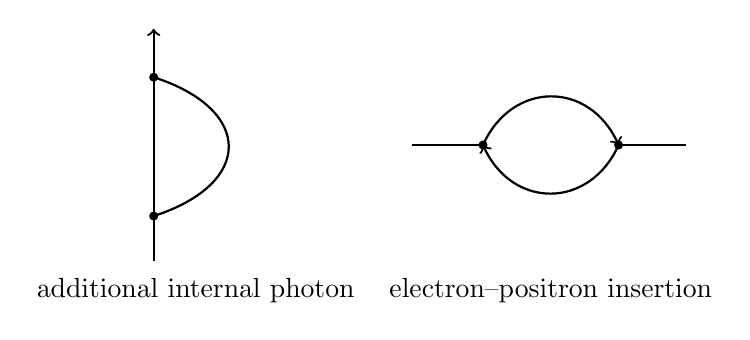
\begin{tikzpicture}[scale=0.82]
\draw[thick,->] (0.9,0.2) -- (0.9,3.8);
\fill (0.9,0.9) circle (2pt);
\fill (0.9,3.05) circle (2pt);
\draw[thick] (0.9,0.9) .. controls (2.45,1.4) and (2.45,2.55) .. (0.9,3.05);
\node at (1.55,-0.25) {additional internal photon};
\begin{scope}[xshift=5.1cm]
\draw[thick] (-0.2,2.0) -- (0.9,2.0);
\fill (0.9,2.0) circle (2pt);
\fill (3.0,2.0) circle (2pt);
\draw[thick,->] (0.9,2.0) .. controls (1.35,3.0) and (2.55,3.0) .. (3.0,2.0);
\draw[thick,->] (3.0,2.0) .. controls (2.55,1.0) and (1.35,1.0) .. (0.9,2.0);
\draw[thick] (3.0,2.0) -- (4.05,2.0);
\node at (1.95,-0.25) {electron--positron insertion};
\end{scope}
\end{tikzpicture}
\caption{بنيتان من رتب أعلى في الديناميكا الكهربائية الكمومية تضيفان رؤوسًا أولية وقوى إضافية من \(e\).}
\end{figure}

وهكذا يمضي التوسع في الديناميكا الكهربائية الكمومية في قوى متعاقبة من \(e^2\). وكل تعقيد جديد مماثل يضيف قوتين من الشحنة الكهربائية إلى السعة. وفي التطبيع المستخدم هنا، يجعل ذلك مثل هذا التصحيح أصغر في السعة بنحو مئة مرة أو بضع مئات المرات من الرتبة السابقة. فالمخططات الأكثر تعقيدًا تضعف تدريجيًا، ولذلك يكون للمجموع الاضطرابي فرصة لأن يكون مفيدًا.

لا يُحصَل على الاحتمال بتربيع كل مخطط على حدة ثم جمع تلك المربعات. بل اجمع أولًا كل سعة تسهم في العملية الخارجية نفسها:
\begin{equation}
\mathcal{A}_{\mathrm{total}}=\sum_r\mathcal{A}_r.
\end{equation}
وعندئذ فقط شكّل
\begin{equation}
P=\left|\mathcal{A}_{\mathrm{total}}\right|^2
=\left|\sum_r\mathcal{A}_r\right|^2.
\end{equation}
أما الحدود المتقاطعة بين المخططات المختلفة فهي حدود تداخل. والقاعدة بسيطة وأساسية: اجمع أولًا، ثم ربِّع.

\section{نحو حصر الجسيمات والنموذج المعياري}

بعد تثبيت المنتشرات، والرؤوس، وعدّ الاقترانات، والتداخل، يمكن أن يبدأ وصف فيزياء الجسيمات على نحو جاد. ويمكن تسمية الجسيمات، وتحديد كتلها، وكتابة اللاغرانجيات التي تحكمها اعتمادًا جزئيًا على النظرية وجزئيًا على التجربة، ودراسة تناظراتها مباشرة في تلك اللاغرانجيات. ثم يقود الإطار نفسه إلى النموذج المعياري وخواصه.

\begin{classroomqa}
\lecturetimestamp{01:33:22}
\audiencequestion{هل يمكن استبدال معامل الكتلة الثابت \(m^2\) بحقل هيغز؟}
\lecturerresponse{نعم. هذه هي الفكرة الصحيحة، وستناقش الآلية لاحقًا.}
\end{classroomqa}

\begin{classroomqa}
\lecturetimestamp{01:33:42}
\audiencequestion{هل يمكن أن تقع نقطتا الشبكة المتجاورتان \(x\) و\(x'\) عند زمنين مختلفين؟}
\lecturerresponse{نعم. قد تكونان متجاورتين في اتجاه الزمن؛ وهكذا يُمثَّل الانتشار الرأسي على الشبكة.}
\end{classroomqa}

بالنسبة إلى النقاط المتجاورة، يحتوي مربع الفروق المنتهية على حدود في الموقع نفسه وحدود ربط بين الموقعين:
\begin{equation}
\bigl[\phi(x)-\phi(x')\bigr]^2
=
\phi(x)^2+\phi(x')^2-2\phi(x)\phi(x').
\end{equation}

\begin{classroomqa}
\lecturetimestamp{01:33:56}
\audiencequestion{أيُّ حدٍّ يمثّل جسيمًا ساكنًا فحسب؟}
\lecturerresponse{تمثّل الحدود في الموقع نفسه \(\phi(x)^2\) و\(\phi(x')^2\) في مربع الفروق المنتهية حالة السكون، بينما يوفّر الحد المتقاطع \(\phi(x)\phi(x')\) تأويل الحركة. كما يساهم حد الكتلة الصريح أيضًا بعوامل في الموقع نفسه تمثل السكون.}
\end{classroomqa}